\RestyleAlgo{boxed}
\chapter{类别层次概率计算模型}
上一章介绍了将预测端的词用二叉树的分层的形式表示,本章将这个目标词表示扩展到类别的形式,并讨论基于类别划分的层次概率模型。首先本章提出在划分的类别结构上建模的单词编码方案,进而推导出该模型的代价函数及其梯度。同时在实验中注意到类别划分的单词分布对模型的性能有很大的影响,应需要在训练阶段之前被定义,所以本文考虑几种现有的词表分割策略,包括:基于单词或者文本的统计、句法和语义知识来划分其层次结构,使模型能达到稳定和高效的结果。在模型推理过程中,本章针对两种不同的情况:1)打分:输出给定序列的概率;2)排序:在给定的上下文中获取得分最高的候选单词,分析并提出可能的优化策略。


\section{词表划分编码}
\begin{table}[!ht]
  \centering
  \caption{并行层次概率计算模型的符号助记表}
\begin{tabular}{llc}
  \toprule
   符号&含义&取值范围\\ \midrule
$\theta^c\in\mathbb{R}^m$ &表示单词的类别向量& Float32\\
$ \theta^o$ &表示路径$l^w$表示划分后的单词三维张量&Float32 \\
$\Gamma'$ &路径查找表,给定单词元组序列,可以获得对应的单词&--- \\
  \bottomrule
\end{tabular}
\end{table}
词表分割算法能将词表划分成多个大小不均匀的分组,传统的类别层次模型仅能计算均匀划分后的单词概率,为了支持广义的词表划分算法,本章提出基于词表划分的元组编码方式。

首先介绍非均匀划分的词表的编码方式,词表被表示成:类别向量~$\theta^c$~和划分的单词矩阵~$\theta^o$。其中前者定义了类别层的概率~$p^c$~,而后者表示该分组内的单词局部概率~$p^o$,如图~\ref{fig:unequal}~所示。其中,划分的单词矩阵的维度是:类维度和分组词维度。如果将词表~$\mathcal{V}$~划分为不等大小的组,则需要将单词矩阵分类为等长矩阵,对于不在这个组中的剩余节点,我们使用零掩码~$\theta^m$来消除其对局部单词概率和总代价函数的影响。
因此,分组词维度是最大的组长度。如果应用词表均匀分割的算法(如图~\ref{fig:equal}~所示),掩码向量~$\theta^m$~可以被忽略,并且分组词维度是~$\mathcal{|V|/|C|}$(~$\mathcal{|C|}$~表示类维度)。另外,如果~$\mathcal{|V|}$~不能被~$\mathcal{|C|}$~整除,那么最后的分组包含实际的单词数量应该小于该组的大小。考虑到这样的不存在的单词占据很少一部分,同时不影响其他类别的概率计算,实际的影响比较小,所以掩码向量~$\theta^m$~可以被忽略。
\begin{equation}\label{equ:partition}
 \theta^m=
\begin{cases}
    \text{单位矩阵,}& \text{若均匀划分} \\
    \text{掩码矩阵,} & \text{否则}
\end{cases}
\end{equation}

\begin{figure}[!ht]
  \centering
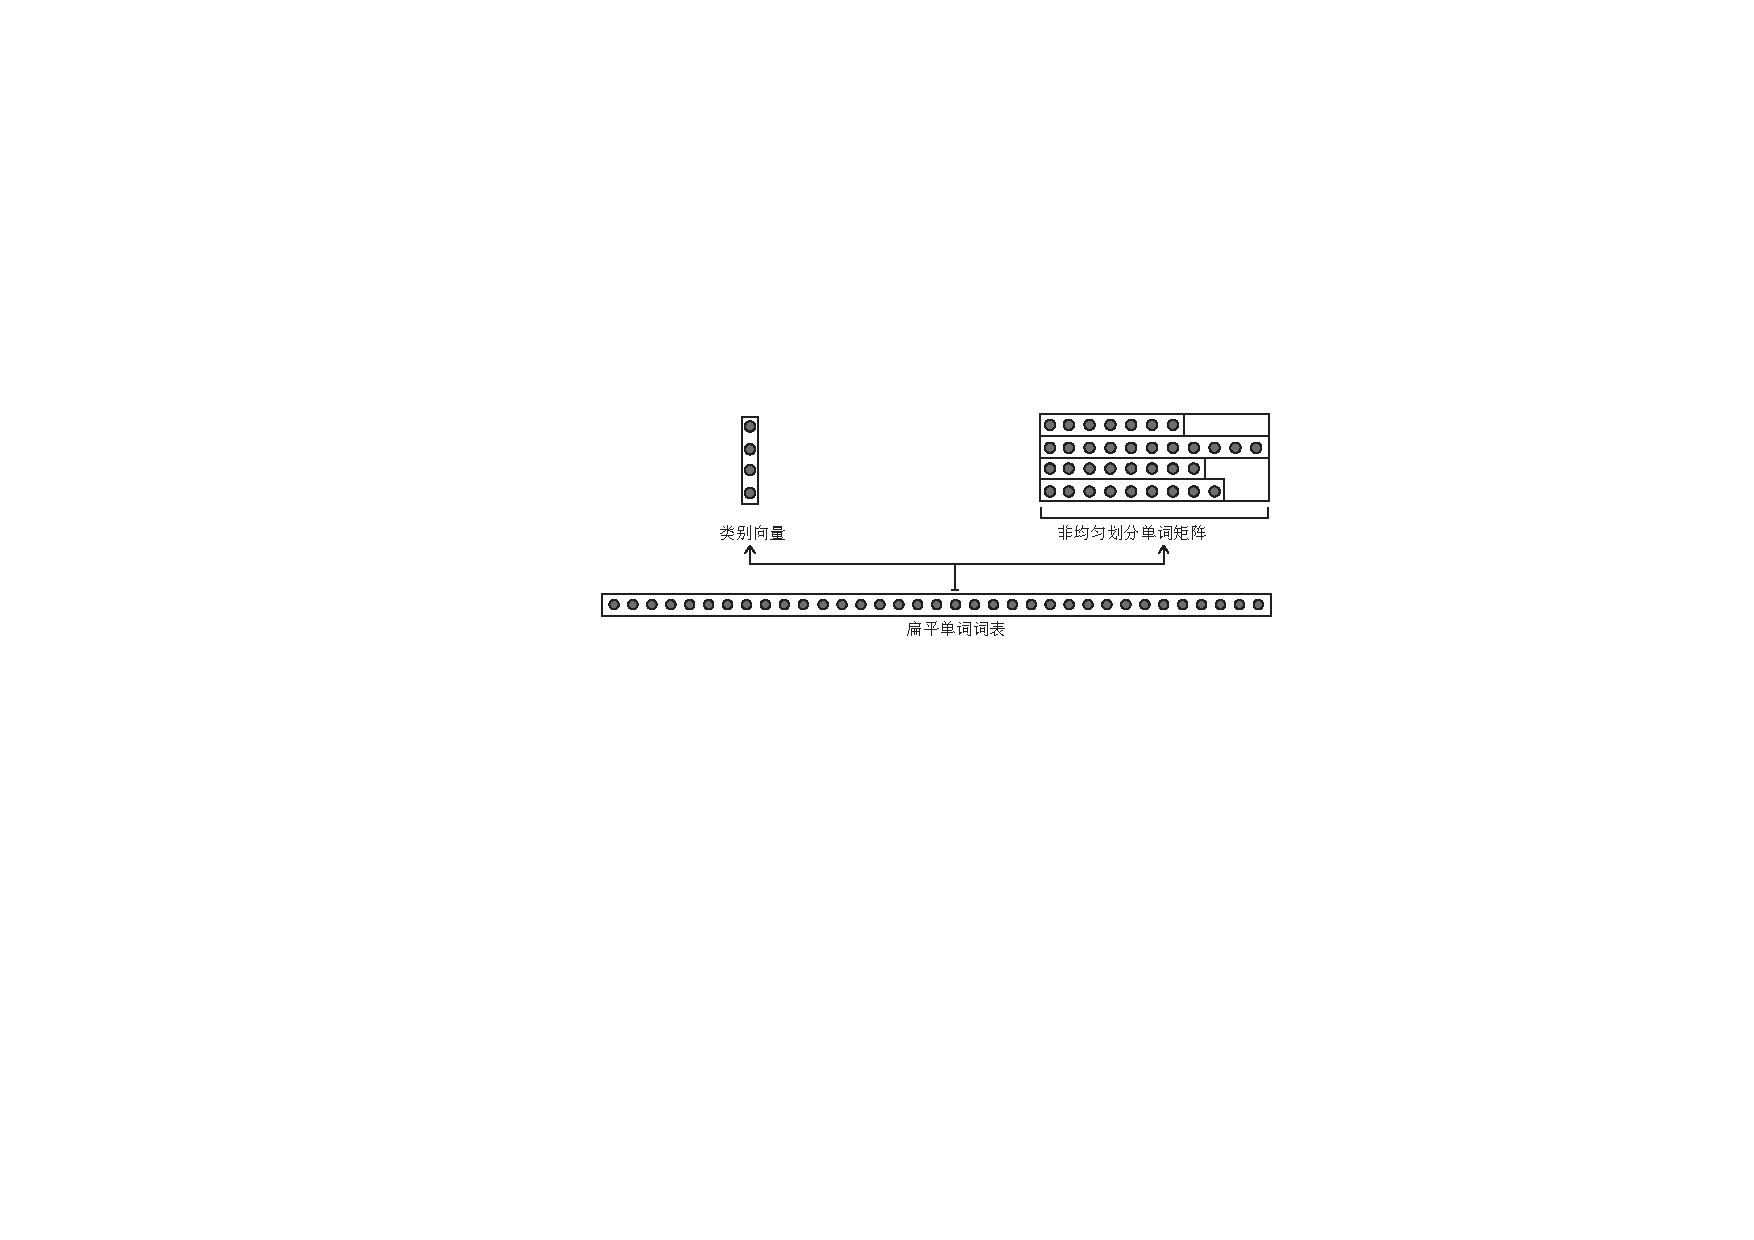
\includegraphics[width=.9\linewidth]{./figures/chsm-simple.pdf}
\caption{非均匀词表划分结构示意图}\label{fig:unequal}
\end{figure}
\begin{figure}[!ht]
  \centering
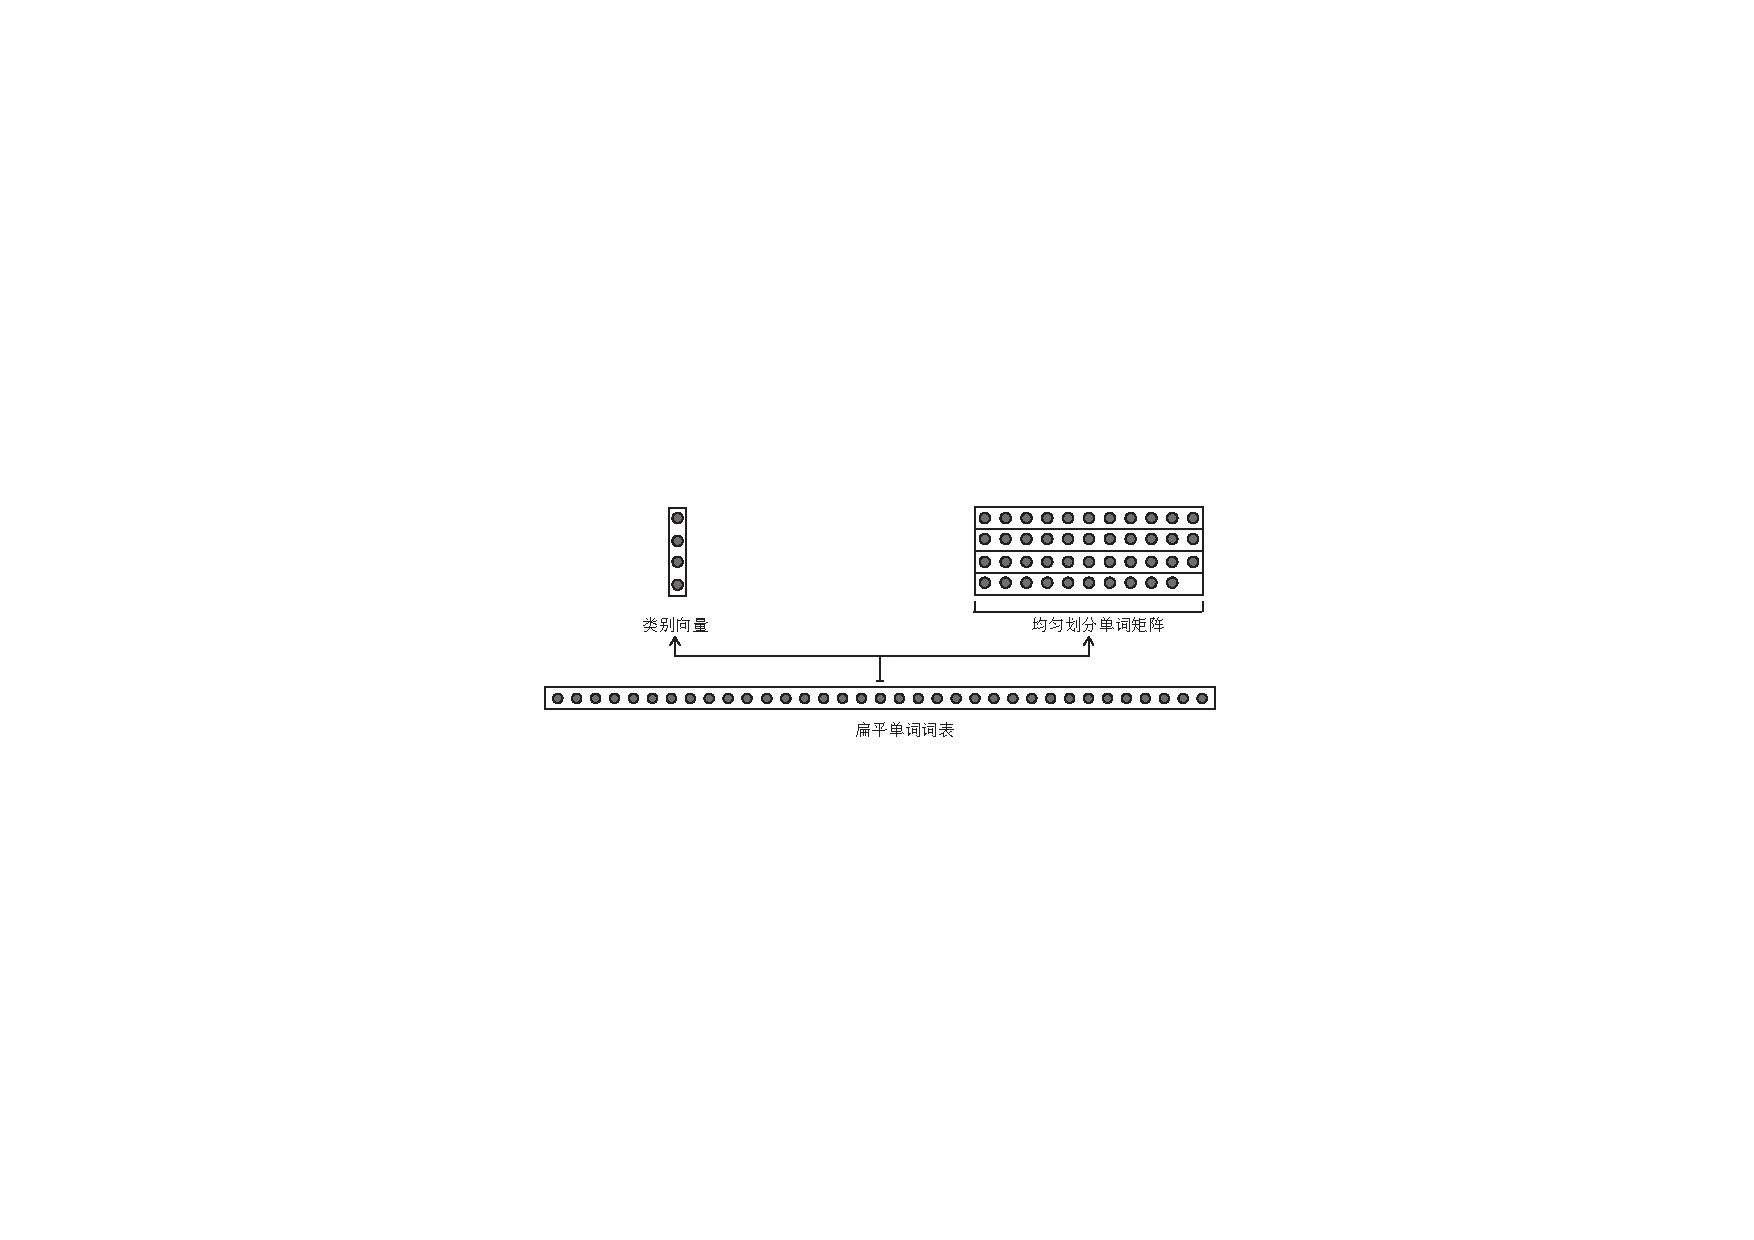
\includegraphics[width=.9\linewidth]{./figures/chsm-simple2.pdf}
\caption{均匀词表划分结构示意图}\label{fig:equal}
\end{figure}

上述的编码方式将一维~1-of-K~的单词索引替换成元组方式的索引~$(w^c,w^o)$,通过该元组可以从预先定预先定义的单词查找表~$\Gamma $~中检索给定单词~$w$,或者给定单词~$w$,通过反向的查找表给出该元组。其中~$w^c$~指代的是单词的类别编号,$w^c$~表示该组内的单词索引。这种编码方式不仅能处理传统的均匀划分词表同时也支持非均匀划分的词表结构。


\section{基于类别的代价函数和导数}
在定义单词基于类别的二元编码后,本章接下来讨论基于这种编码的代价函数和导数计算公式。
给定隐藏层输出向量~$h$,那么该分组中的每个组和和该分组中单词的局部概率可以被定义为:
\begin{equation}
\begin{split}
\log p^c(c|h) &= \theta^c h-\log \sum{\exp( \theta^c h )} \\
\log p^o(w|w^c,h)&=\theta^o h -\log\sum\exp{(\theta^o h)}
\end{split}
\end{equation}
其中~$p^c$~和~$p^o$~是分别计算而不是同时计算的。因为主要的计算瓶颈在单词局部概率~$p^o$~中,所以主要问题是减少第二项概率的计算量而不是同时计算这两项概率。因此本文的主要工作集中在如何高效计算~$p^o$。例如,假设我们将词表大小为~10000~的单词均匀划分,那么类别向量的维度是~100,单词矩阵的维度是~$[100,100]$。如果两者能够同时计算,而不是依次计算,它所带来的计算效率增益可以如下计算:
\begin{equation}\label{equ:example}
  \frac{\frac{1}{100*100}}{\frac{1}{100*100+100}}-1=1\%
\end{equation}
从上面的计算结果来看,我们只能提升~$1/\%$~的速度方面性能。那么如果每次只计算对应单词的单词矩阵的概率值,计算效率可以如下计算:
\begin{equation}\label{equ:example2}
  \frac{\frac{1}{100+100}}{\frac{1}{100*100+100}}-1=49.5
\end{equation}
可以发现,只要能避免计算全局概率就能实现~$49.5$~倍的计算效率增益。使用分类的层次概率模型能直接将模型的计算瓶颈削弱到很少计算时间,尽管相比于树状模型该模型的计算速度不是最快的。除此之外,基于类别的层次概率模型的优点包括:1)模型鲁棒性更强,单词的分组分布对模型的精确度影响比树状层次概率模型小;2)模型实现容易,通用性强。只需要将所有单词划分几个分组即可,不需要做层次二叉聚类算法,而且层次二叉聚类算法计算时间复杂度相当高,不适合实际使用。



在介绍完模型的类别编码方式中提及的掩码向量并不是直接应用于这个分词矩阵,而是应用在对数概率归一化(log softmax)的计算步骤中。 举例来说,在~softmax~函数中:$p(x_i)={\exp({x_i}})/{\sum_j\exp(x_j)}$,如果~$x_k=0$,然而其概率值~$p(x_k)>0$~,这是因为~$\exp(x_k)>0$。即:在该类别中不存在的单词,仍然有概率数值和概率分布,这样对于那些实际存在的单词概率来说,至多有~$\mathcal{|V|/\mathcal{C}}-1$~的类别概率被稀释,这被称为概率稀释问题。因此,该组中正确的的局部单词的对数概率计算如下:
\begin{equation}
  \log \tilde p^o(w|w^c,h)=\theta^o h -\log\sum\theta^m\exp(\theta^o h)
\end{equation}
其中~$\theta^m\exp(\theta^o h)$~保证了那些不存在的单词经过掩码向量之后数值是~0,从而不会对公示的第二项产生影响。

接下来推导模型的代价函数,模型的预测损失主要来自两项:类别预测错误和分组中的单词预测错误,所以该层次模型的损失函数可以从这两项错误分类中算出,可以写成如下的形式:
\begin{equation}
\ell(\theta|h) =\log p^c(w^c|h) +\log \tilde  p^o(w^o|w^c,h)
\end{equation}
其中计算$\log \tilde  p^o(w^o|w^c,h)$,需要指定其类别~$w^c$。在模型训练过程中,$w^c$~是需要预先定义的,在测试过程中,需要同时考虑 ~$p^c$~和 ~$p^o$~两项概率,才能选择概率最大的单词,单独计算$\arg\max p^c$~和 ~$\arg\max p^o$~均无法获得概率最大的单词。

总的来说,将词表分成相互排斥的分组的优点可以概括为:1)避免了在整个词表上计算归一化(Normalization)概率。 由于~$p^c$~是在类维度上计算概率归一化概率,$p^o$~是在最大组大小维度上计算归一化概率。 所以在第二个方程中,其他分组中的单词被忽略不需要计算,其中~$\mathcal{|C|}$~和~$\mathcal{|V|}/\mathcal{|C|}$~在最大的实验数据集都不会超过~1000; 2)与基于二叉树结构相比,它对词表的结构约束(Structural Constraint)更少,在分层预测过程中丢失的信息更少;3)与单词拆分方法相比,它不会增加序列长度,所以不会影响循环网络的长距离依赖的建模问题。

当定义模型的代价函数之后,接下来推导得模型所涉及的参数的导数,以便于模型求解优化。模型的所有的参数包括:$\{\theta^c,\theta^o,h\}$,模型的代价函数对于这些参数的导数计算公式如下:
\begin{equation}
\begin{split}
\frac{\partial \ell}{\partial \theta^c}=& (\delta_{ij}-p(c|h))h \\
\frac{\partial \ell}{\partial \theta^o}=&(\delta_{ij}-p(w|c,h))h \\
\frac{\partial \ell}{\partial h}=&(\delta_{ij}-p^c(c|h))\theta^c + (\delta_{ij}-p^o(w|c,h))\theta^o
\end{split}
\end{equation}


\section{基于类别的测试推理}
在推理测试阶段,对于类别的层次概率模型来说,序列的概率直接运用模型的代价函数计算获得,如下所示:
\begin{equation}\label{equ:class_inf}
\log p(w_1,\cdots, w_T)=\sum_t^T\log p(w_t|h_t) =\sum_{t=1}^{T}\log p^c(w^c_t|h_t) +\log p^o(w^o_t|w^c_t,h_t)
\end{equation}
该方法的计算复杂度~$\mathcal{O(|H|\sqrt{|\mathcal{V}|})}$~,比softmax函数计算效率更高,两者的加速比是~$|\mathcal{V}|/\sqrt{|\mathcal{V}|}$。

\begin{algorithm}[!ht]
\caption{基于 cHSM 算法的全局 $\arg\max$ 算法}\label{algo:alls}
\KwData{ 隐藏层输出 $h$}
 \For{$c \in \mathcal{C}$ }{
 {// 计算类别的概率~$\log p^c(c|h)$}\;
 {$\log p^c(c|h) = \theta^c h-\log \sum{\exp( \theta^c h )}$}\;
 \For{w $\in$ c}{
 {// 计算单词的条件概率~$\log p^o(\hat w^o|\hat y^c,h)$}\;
 {$ \log \tilde p^o(w|w^c,h)=\theta^o h -\log\sum\theta^m\exp(\theta^o h)$}\;
 {// 计算每个单词全局概率}\;
  {$\log p(w|h)=\log p^c(w^c|h)+\log \tilde p^o(\hat w^o|\hat w^c,h)$}\;
 }
 }
 {$w=\arg\max_w \log p(w|h)$}\;
 \KwResult{概率最大的候选单词$w$。}
\end{algorithm}

其次对于第二种词表排序的情况,首先可以计算词汇表中所有单词的概率,然后调用排序函数,从而选择概率最高的单词,如算法~\ref{algo:alls}~所示。 此外,我们仍然可以在算法~\ref{alog:exact}~中对上述方法进行少量修改,然后计算全局概率最佳的单词。两者的差异是,算法~\ref{alog:exact}~最后的$\arg\max$的计算量是~$\mathcal{|C|}$,算法~\ref{alog:exact}~最后的$\arg\max$的计算量是$\mathcal{|V|}$。
\begin{algorithm}[!t]
\caption{基于 cHSM 算法的正确 $\arg\max$ 算法}\label{alog:exact}
\KwData{ 隐藏层输出 $h$}
{// 挑选每个类中概率最大的类别}\;
 {$\hat w^o=\arg\max_o{\log p^o(w| c,h)}$ }\;
 {// 在这些已经被栅选单词中挑选最佳的单词}
 {$\tilde w^c=\arg\max_c{\log p^c(w^c|h)+\log p^o(\hat w^o|\hat y^c,h)}$}\;
通过查找表 $\Gamma'$ 将 $(\tilde w^c,\hat w^o[\tilde w^c])$替换成单词$w$ \;
 \KwResult{概率最大的候选单词$w$。}
\end{algorithm}


此外,cHSM算法的性能对词表划分算法有些敏感,因为某些方法可能会产生高度不平衡的字组,并且这种单词不均匀分布会在算法中产生标签偏差问题(Label Bias)。第一个本地~$\arg\max_o$~进程~\upcite{DBLP:conf/icml/LaffertyMP01}。然而,在大多数情况下,如果选择合适的参数,则可以考虑不平衡的问题,本文考虑平衡词汇分区的广义形式。

我们接下来来详细说明标签偏差问题。考虑两个类~$c_p$~和~$c_q$,这两个类的包含的单词数量是不同的,我们不妨假设~$|c_p|\le|c_q|$。在计算了最后一个隐藏层输出~$h$~与类图层参数的相似性之后,我们继续计算~$h$~与每个组的内部单词~$w$ 的相似性得分,这些单词在每个特定组中都没有进行局部规范化整个词汇。当~$|c_p|\approx|c_q|$~表示我们希望将词汇聚类成等大小的群组,而不是高度倾斜的群组分布时,可以减轻标签偏差问题,其中~$|c_p|\ll|c_q|$ 。更具体地说,对于分布不均的情况,对于类~$c_q$~中的单词来说这个概率被一大群单词稀释是不公平的,这样算法更有可能以较高的概率取出这个小组中的单词,放弃在其他大集团有更多的潜在的话。

我们可以用局部贪心算法搜索次优结果,而不是搜索确切的全局最优结果,而是建议将这个~$\arg\max$~进程分解为两个阶段:1)计算类概率,并剔除顶端一个~$\hat c$; 2)计算该类别的单词概率~$\hat c$,并选择具有最高本地单词概率的单词。这个算法会给psudo最好的候选人,但是与原始算法~\ref{alog:exact}相比,它的运行速度要快得多。而且,由于分组词在本地进行归一化,标签偏差问题可以在一定程度上缓解。在实验研究中将讨论算法~\ref{alog:exact}~和~\ref{alog:cargmax}~的详细不同性能。
\begin{algorithm}[!t]
 \caption{基于 cHSM 模型伪~$\arg\max$~算法}\label{alog:cargmax}
\KwData{隐藏层输出 $h$;}
{// 挑选概率最大的类别}\;
 {$\hat w^c=\arg\max_c{\log p^c(c|h)}$ }\;
 {$\hat w^o=\arg\max_o{\log p^o(w|\hat w^c,h)}$}\;
 {// 在这个类别下面,挑选概率最大的单词}\;
 {通过查找表 $\Gamma'$ 将 $(\hat w^c,\hat w^o)$替换成单词$w$}\;
 \KwResult{ 最佳的候选单词 $\hat w$.}
\end{algorithm}

\section{词表划分算法}
由于cHSM模型的性能与其词汇分割算法密切相关,我们将聚类算法的现有工作进行汇总,并将可能的方法分类如下:

\subsection{均匀词表划分算法}
1) 随机初始化。 这种直观的方法忽略了单词的所有外部信息,因此单词与随机随机播放过程是等分的。这是揭示其他聚类方法下界的最坏情况,也可以揭示应用高级聚类策略的相对收益。

2) 字母顺序。这种方法根据字符级别的信息对单词进行排序,同一组中的单词共享一个相似的子字符串。

3) 一元单词聚类。这些单词首先根据它们在文本中的频率排序,然后通过放置边界使得每个类别占总概率质量的恒定部分,从而形成连续单词块。这种方法具有这样的性质:较低编号的类比较高编号的类具有更少的成员,因为它们的成员更频繁~\upcite{DBLP:conf/nips/MikolovSCCD13}。


\subsection{非均匀词表划分算法}
1) 二元单词聚类。它是指布朗聚类方法,这是历史适用于基于n-gram的基于类的模型~\upcite{DBLP:journals/coling/BrownPdLM92,liang2005semi}。单词使用相同的bigram上下文分组到相同的行中。

2) 结构聚类\footnote{https://github.com/AlonDaks/unsupervised-authorial-clustering}。根据文本中的单词的词性和句法结构划分词表~\upcite{DBLP:conf/acl/DaksC16} 。

3) 语义聚类。我们将传统的kmeans聚类方法应用到预训练的词嵌入,使得我们可以通过指定聚类的大小将词汇分成不同的形状。

\section{本章小结}
本章首先定义了基于词表划分的编码概念,同时给出了模型所涉及的参数的详细涵义。接下来,我们逐步推导模型的单个节点的概率公式,单个词的概率公式和模型的代价函数。另一方面,我们将提出的p-cHSM算法和传统的线性cHSM算法进行的比较。通过比较两者计算的差异性证明我们提出的算法更适合在GPGPU等高并行设备上运算。进一步的,我们还讨论了模型在测试的时候所需的推理算法,因为基于划分词表的概率计算方案和传统的softmax计算方案不同,不能直接输出单个词的概率或者计算最佳的候选单词,所以我们分别针对这两个任务提出推理算法。最后,由于单词在单词划分矩阵上的分布需要初始化,我们讨论了传统的霍夫曼硬聚类算法,布朗软聚类算法和语义向量软聚类算法等等。同时也讨论三种算法的实际应用过程。